\chapter{Internet Principles}



\section{Section 1: Internet Communications and the TCP/IP Suite}

\subsection{1. Introduction to Internet Communications}
Internet communications form the backbone of the Internet of Things, enabling heterogeneous devices (sensors, gateways, servers) to exchange data globally. IoT leverages the existing TCP/IP architecture to ensure interoperability across diverse hardware platforms and physical transmission media.

\subsection{2. TCP/IP Protocol Suite vs. OSI Reference Model}
The \textbf{OSI (Open Systems Interconnection) Model} is a theoretical 7-layer framework developed by ISO, whereas the \textbf{TCP/IP Suite} is a practical 4-layer architecture implemented in real-world networking.

\begin{figure}[H]
\centering
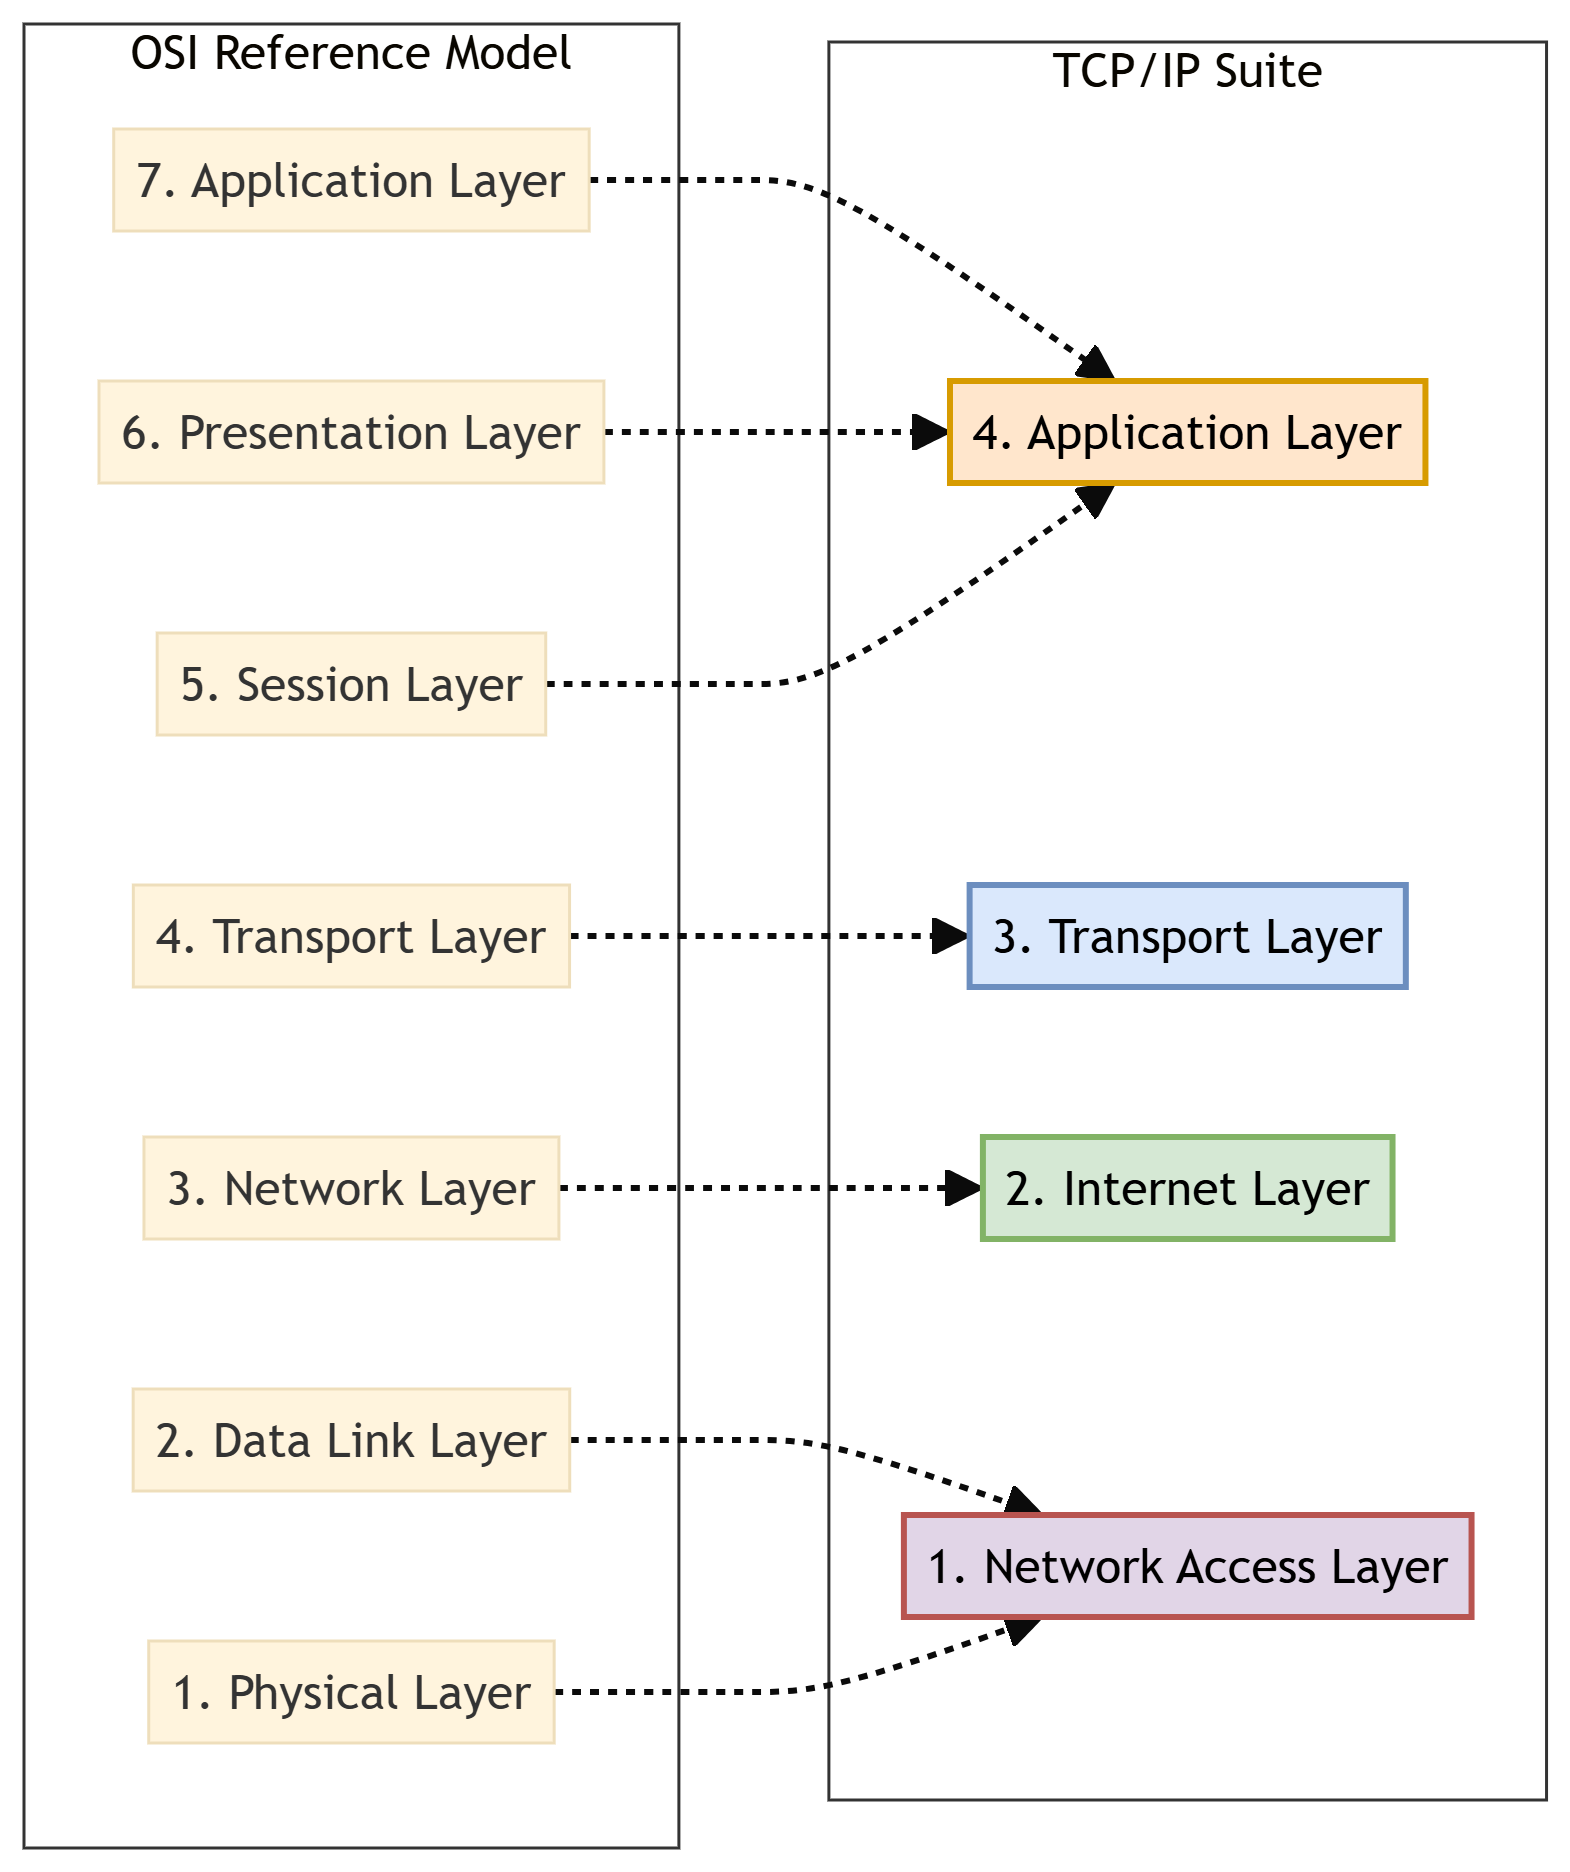
\includegraphics[width=0.75\textwidth,height=0.32\textheight,keepaspectratio]{../Images/chapter_03/tcp_ip_vs_osi.png}
\caption{TCP/IP Suite vs. OSI Reference Model Mapping}
\end{figure}

\subsection{3. Detailed Layer Comparison and Protocol Examples}

\begin{table}[H]
\centering
\begin{tabular}{|p{\dimexpr 0.18\textwidth - 2\tabcolsep - 1.5\arrayrulewidth\relax}|p{\dimexpr 0.27\textwidth - 2\tabcolsep - 1.5\arrayrulewidth\relax}|p{\dimexpr 0.27\textwidth - 2\tabcolsep - 1.5\arrayrulewidth\relax}|p{\dimexpr 0.28\textwidth - 2\tabcolsep - 1.5\arrayrulewidth\relax}|}
\hline
TCP/IP Layer & Corresponding OSI Layer(s) & Primary Responsibility in IoT & Standard IoT/Internet Protocols \\
\hline
\textbf{4. Application} & Application (7), Presentation (6), Session (5) & Formats data, manages sessions, and defines client-server or pub/sub communication models. & HTTP, CoAP, MQTT, DNS, DHCP \\
\hline
\textbf{3. Transport} & Transport (4) & Establishes host-to-host connectivity, error checking, flow control, and packet sequencing. & TCP, UDP \\
\hline
\textbf{2. Internet} & Network (3) & Handles logical addressing, routing packets across multiple networks, and fragmentation. & IPv4, IPv6, ICMP, 6LoWPAN \\
\hline
\textbf{1. Network Access} & Data Link (2), Physical (1) & Defines physical media access (cables/radio waves), physical addressing, and framing. & Ethernet (802.3), Wi-Fi (802.11), BLE, Zigbee \\
\hline
\end{tabular}
\end{table}


\section{Section 2: Bluetooth Low Energy (BLE) (Q3.1) [5M]}

\subsection{1. Definition and Core Features}
\textbf{Bluetooth Low Energy (BLE)} (introduced in Bluetooth 4.0 as Bluetooth Smart) is a wireless personal area network (WPAN) technology designed by the Bluetooth Special Interest Group (SIG) specifically for low-power, low-latency, and low-data-rate short-range communications.

\subsubsection{Core Features:}
\begin{itemize}
  \item   \textbf{Ultra-Low Power Consumption:} Devices can run for months or years on a single coin-cell battery (e.g., CR2032) by spending most of their time in a deep \textbf{sleep state}.
  \item   \textbf{Fast Connection Setup:} Connection establishment takes less than \textbf{3 milliseconds} (compared to 6 seconds in Classic Bluetooth), minimizing active RF radio uptime.
  \item   \textbf{Advertising Mode:} BLE devices can broadcast short packets of data ("advertisements") without establishing a formal connection, allowing quick sensor readouts (beacons).
  \item   \textbf{GATT (Generic Attribute Profile) Structure:} Organizes data hierarchically into Profiles, Services, and Characteristics, allowing standard read/write operations.
\end{itemize}


\subsection{2. Comparison: Classic Bluetooth vs. Bluetooth Low Energy (BLE)}

\begin{table}[H]
\centering
\begin{tabular}{|p{\dimexpr 0.2\textwidth - 2\tabcolsep - 1.5\arrayrulewidth\relax}|p{\dimexpr 0.4\textwidth - 2\tabcolsep - 1.5\arrayrulewidth\relax}|p{\dimexpr 0.4\textwidth - 2\tabcolsep - 1.5\arrayrulewidth\relax}|}
\hline
Feature / Criteria & Classic Bluetooth (BR/EDR) & Bluetooth Low Energy (BLE) \\
\hline
\textbf{Primary Design Goal} & High-throughput continuous data stream. & Low duty cycle, ultra-low power consumption. \\
\hline
\textbf{Power Consumption} & High (1 Watt reference; active battery drain). & Ultra-low (0.01 to 0.05 Watts; sleeping mostly). \\
\hline
\textbf{Data Rate (Throughput)} & 1 to 3 Mbps. & 125 Kbps to 2 Mbps. \\
\hline
\textbf{Connection Setup Latency} & Up to 6 seconds. & Under 3 milliseconds. \\
\hline
\textbf{Voice / Audio Capability} & Supported (ideal for headsets/speakers). & Not natively designed for continuous audio (only BLE Audio). \\
\hline
\textbf{Network Topology} & Piconet (1 Master, max 7 active Slaves). & Scatternet \& Mesh (unlimited nodes in Mesh). \\
\hline
\textbf{Operational State} & Always active / standby modes. & Sleep state by default, wakes up only to transmit. \\
\hline
\end{tabular}
\end{table}


\subsection{3. Advantages and Disadvantages of BLE in IoT}

\subsubsection{Advantages:}
\begin{enumerate}
  \item \textbf{Extended Battery Life:} Fits coin-cell powered wearable medical patches and smart home sensors perfectly.
  \item \textbf{Low Hardware Cost:} Radio chips are highly integrated, small, and inexpensive.
  \item \textbf{Smartphone Integration:} Supported by almost all modern smartphones, eliminating the need for an external gateway.
\end{enumerate}

\subsubsection{Disadvantages:}
\begin{enumerate}
  \item \textbf{Low Data Rates:} Inadequate for streaming video, images, or large files.
  \item \textbf{Short Range:} Typical indoor coverage is limited to 10–30 meters.
  \item \textbf{Incompatibility:} Not backward compatible with legacy Classic Bluetooth hardware.
\end{enumerate}


\section{Section 3: IP Addressing \& DHCP (Q3.2) [5M]}

\subsection{1. Static vs. Dynamic IP Addressing}

\begin{table}[H]
\centering
\begin{tabular}{|p{\dimexpr 0.2\textwidth - 2\tabcolsep - 1.5\arrayrulewidth\relax}|p{\dimexpr 0.4\textwidth - 2\tabcolsep - 1.5\arrayrulewidth\relax}|p{\dimexpr 0.4\textwidth - 2\tabcolsep - 1.5\arrayrulewidth\relax}|}
\hline
Addressing Method & Static IP Addressing & Dynamic IP Addressing \\
\hline
\textbf{Definition} & Manually configured and permanently assigned to a network interface. & Automatically assigned by a network server for a temporary duration. \\
\hline
\textbf{Ease of Configuration} & High overhead; requires manual entry on every device. & Zero-touch configuration for the client device. \\
\hline
\textbf{IP Reusability} & None; the IP remains reserved even if the device is offline. & High; inactive IPs return to the address pool. \\
\hline
\textbf{Security Risk} & Higher risk of targeted attacks as the IP never changes. & Lower risk; IP changes periodically. \\
\hline
\textbf{Ideal IoT Use Case} & Network gateways, local MQTT brokers, and central servers. & Edge sensor nodes, smart bulbs, and mobile clients. \\
\hline
\end{tabular}
\end{table}


\subsection{2. Working Principle of DHCP: The DORA Handshake}
The \textbf{Dynamic Host Configuration Protocol (DHCP)} is an application layer protocol that automates the assignment of IP addresses, subnet masks, default gateways, and DNS server IPs.

The standard transaction uses a four-step process known as \textbf{DORA}:

\begin{figure}[H]
\centering
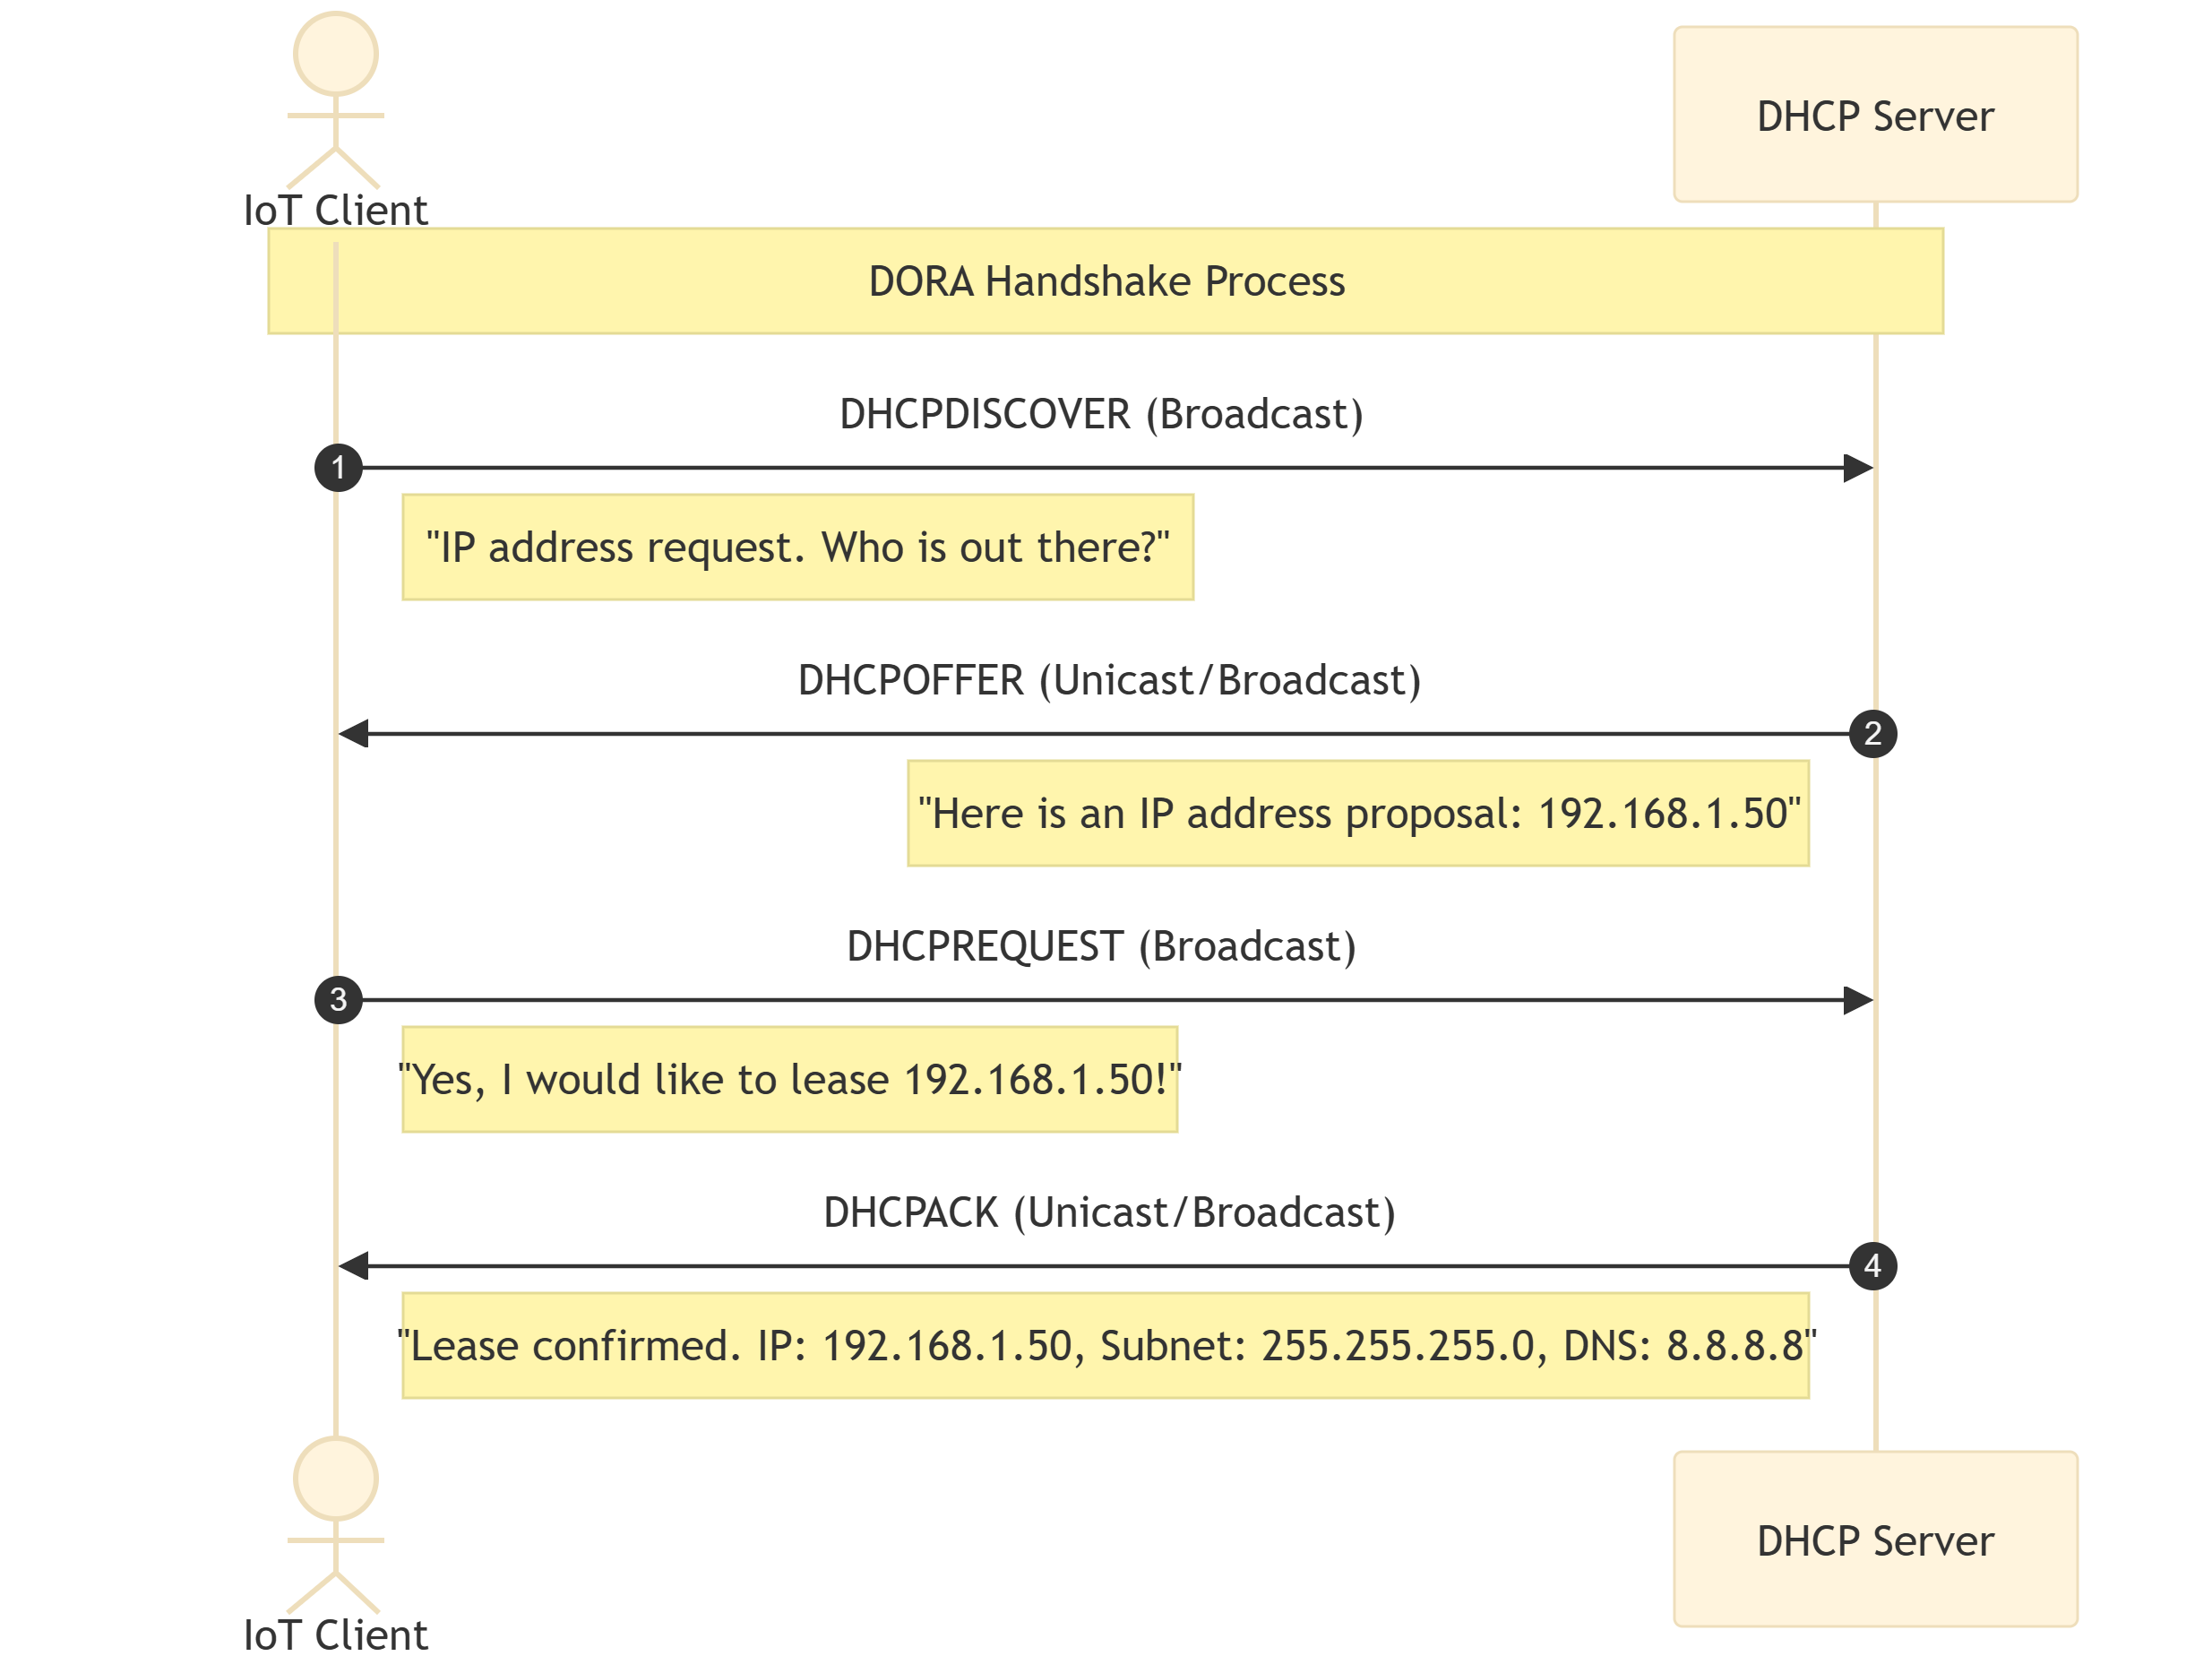
\includegraphics[width=0.75\textwidth,height=0.32\textheight,keepaspectratio]{../Images/chapter_03/dhcp_handshake.png}
\caption{DHCP DORA Handshake}
\end{figure}

\begin{enumerate}
  \item \textbf{DHCPDISCOVER (D):}
\end{enumerate}
\begin{itemize}
  \item   \textbf{Action:} The client broadcasts a message to find any available DHCP server.
  \item   \textbf{Source IP:} `0.0.0.0` | \textbf{Destination IP:} `255.255.255.255` (Broadcast).
\end{itemize}
\begin{enumerate}
  \item \textbf{DHCPOFFER (O):}
\end{enumerate}
\begin{itemize}
  \item   \textbf{Action:} Any receiving DHCP server reserves an IP address and unicasts/broadcasts a proposal containing an IP address, lease time, subnet mask, and DNS information.
\end{itemize}
\begin{enumerate}
  \item \textbf{DHCPREQUEST (R):}
\end{enumerate}
\begin{itemize}
  \item   \textbf{Action:} The client broadcasts a message accepting the proposal from a specific server, notifying other servers that their offers were declined.
\end{itemize}
\begin{enumerate}
  \item \textbf{DHCPACK (A):}
\end{enumerate}
\begin{itemize}
  \item   \textbf{Action:} The server sends a confirmation packet. The client configures its network interface with the leased parameters.
\end{itemize}


\subsection{3. Network Example of DHCP Working}
Consider a \textbf{Smart Thermostat} boot-up sequence in a home network:
\begin{enumerate}
  \item On boot, the thermostat has no IP configuration. It broadcasts a `DHCPDISCOVER` packet over Wi-Fi.
  \item The home Wi-Fi Router (acting as the DHCP Server) receives this and checks its address pool. It replies with a `DHCPOFFER` proposing the IP `192.168.1.15` for a lease time of 24 hours.
  \item The thermostat replies with a `DHCPREQUEST` confirming it wants `192.168.1.15`.
  \item The router logs the MAC address of the thermostat against `192.168.1.15` and transmits a `DHCPACK`. The thermostat is now online.
\end{enumerate}


\subsection{4. Domain Name System (DNS) in IoT}
\begin{itemize}
  \item   \textbf{Concept:} IoT devices typically connect to cloud servers using human-readable domain names (e.g., `api.thingspeak.com` or `mqtt.eclipseprojects.io`) rather than hardcoded IP addresses. The \textbf{Domain Name System (DNS)} is a hierarchical distributed naming system that resolves these domain names into numeric IP addresses (IPv4 or IPv6) that routers use to forward data packets.
  \item   \textbf{Resolution Process:} As shown in the sequence below, the device queries a local DNS resolver, which recursively queries Root, Top-Level Domain (TLD), and Authoritative nameservers until the target IP is returned and cached.
\end{itemize}

\begin{figure}[H]
\centering
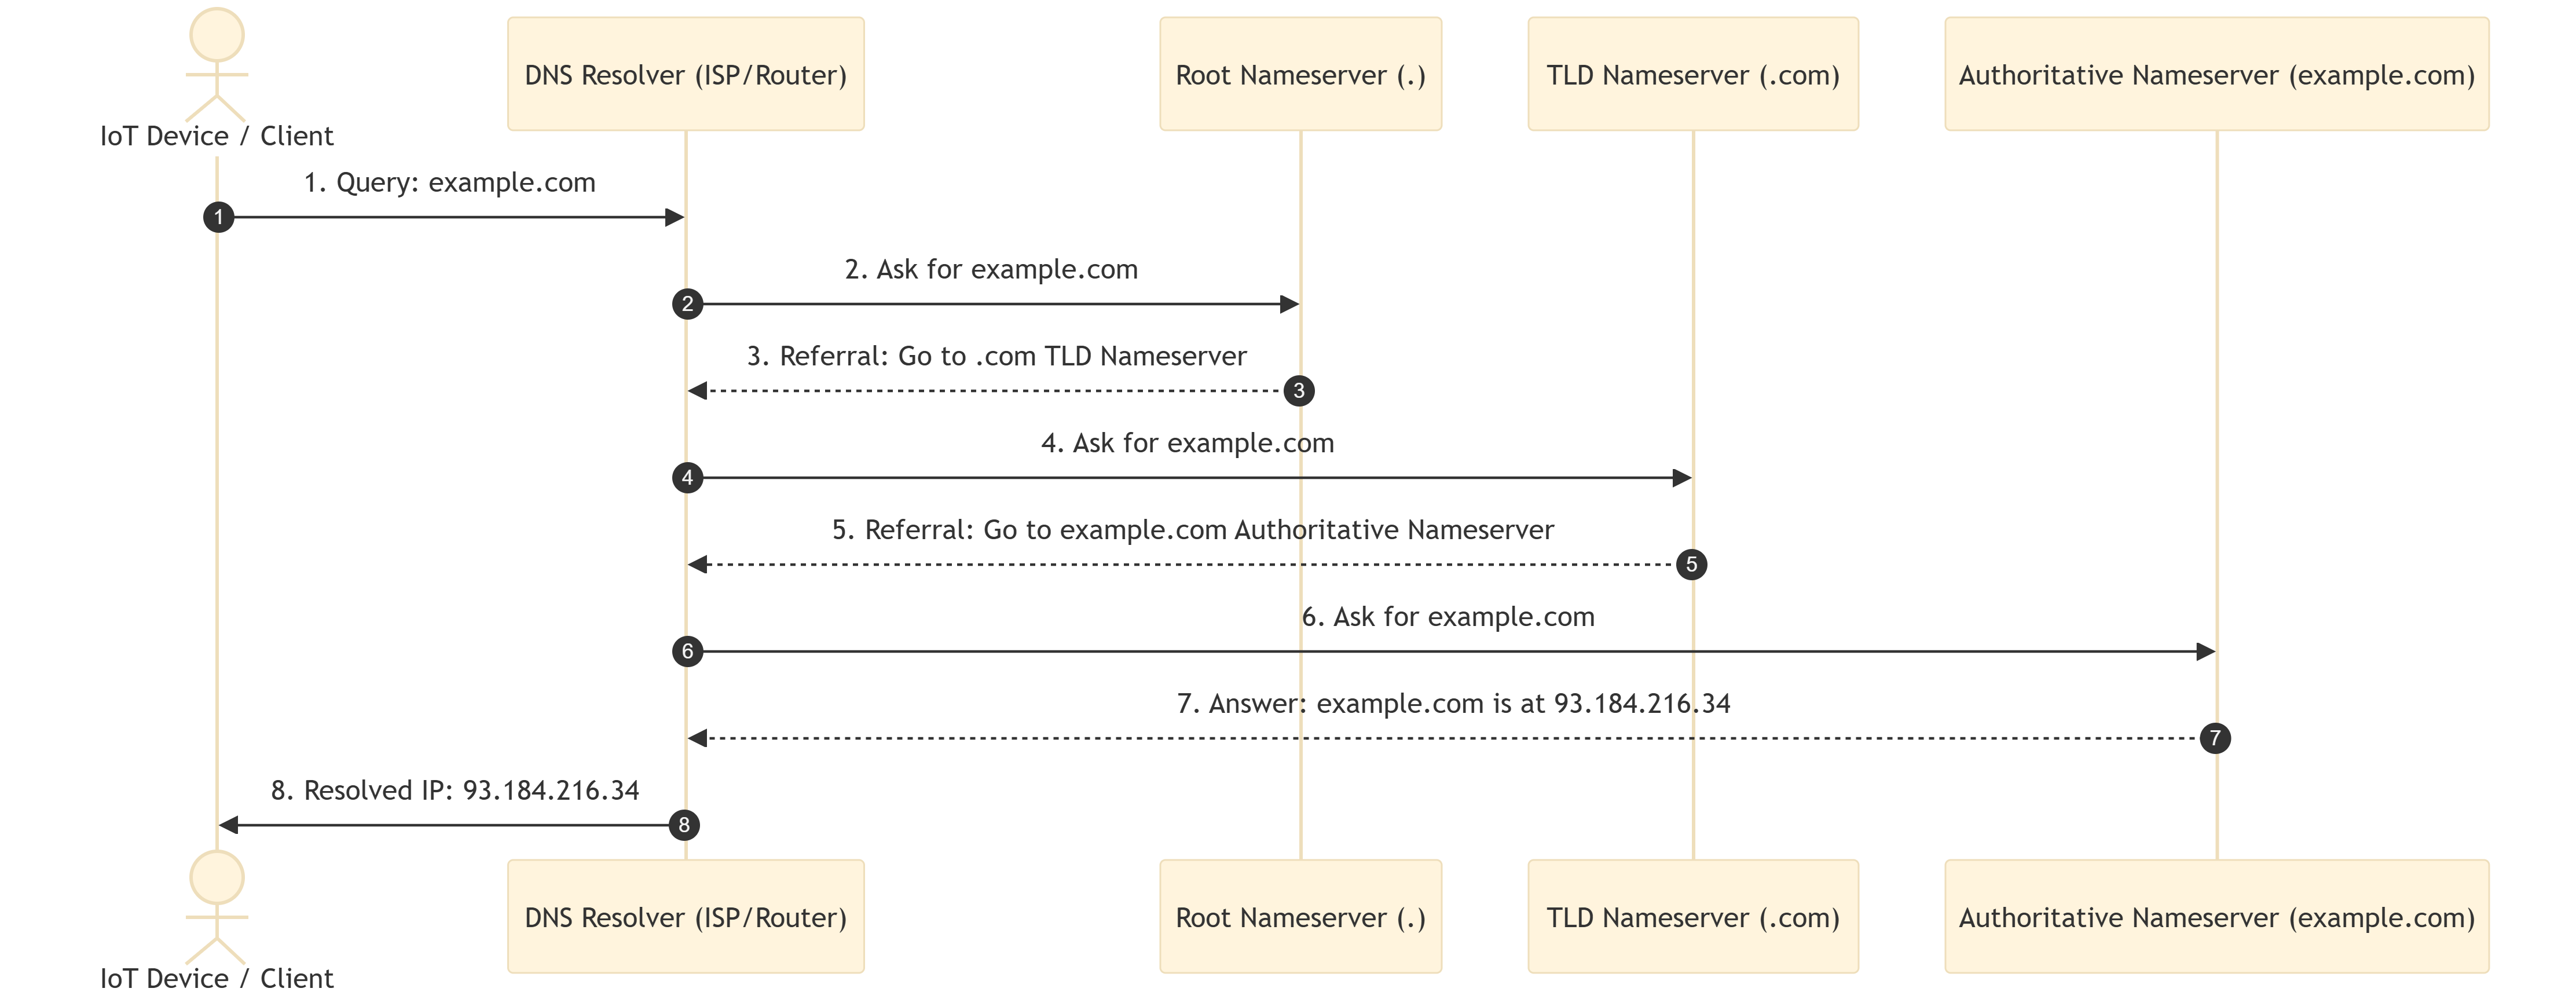
\includegraphics[width=0.75\textwidth,height=0.32\textheight,keepaspectratio]{../Images/chapter_03/dns_resolution.png}
\caption{DNS Resolution Process}
\end{figure}


\section{Section 4: TCP vs. UDP Transport Layer Protocols (Q3.3) [5M]}

The Transport Layer manages how data is shipped across network endpoints. IoT uses two primary protocols: \textbf{TCP (Transmission Control Protocol)} and \textbf{UDP (User Datagram Protocol)}.

\begin{figure}[H]
\centering
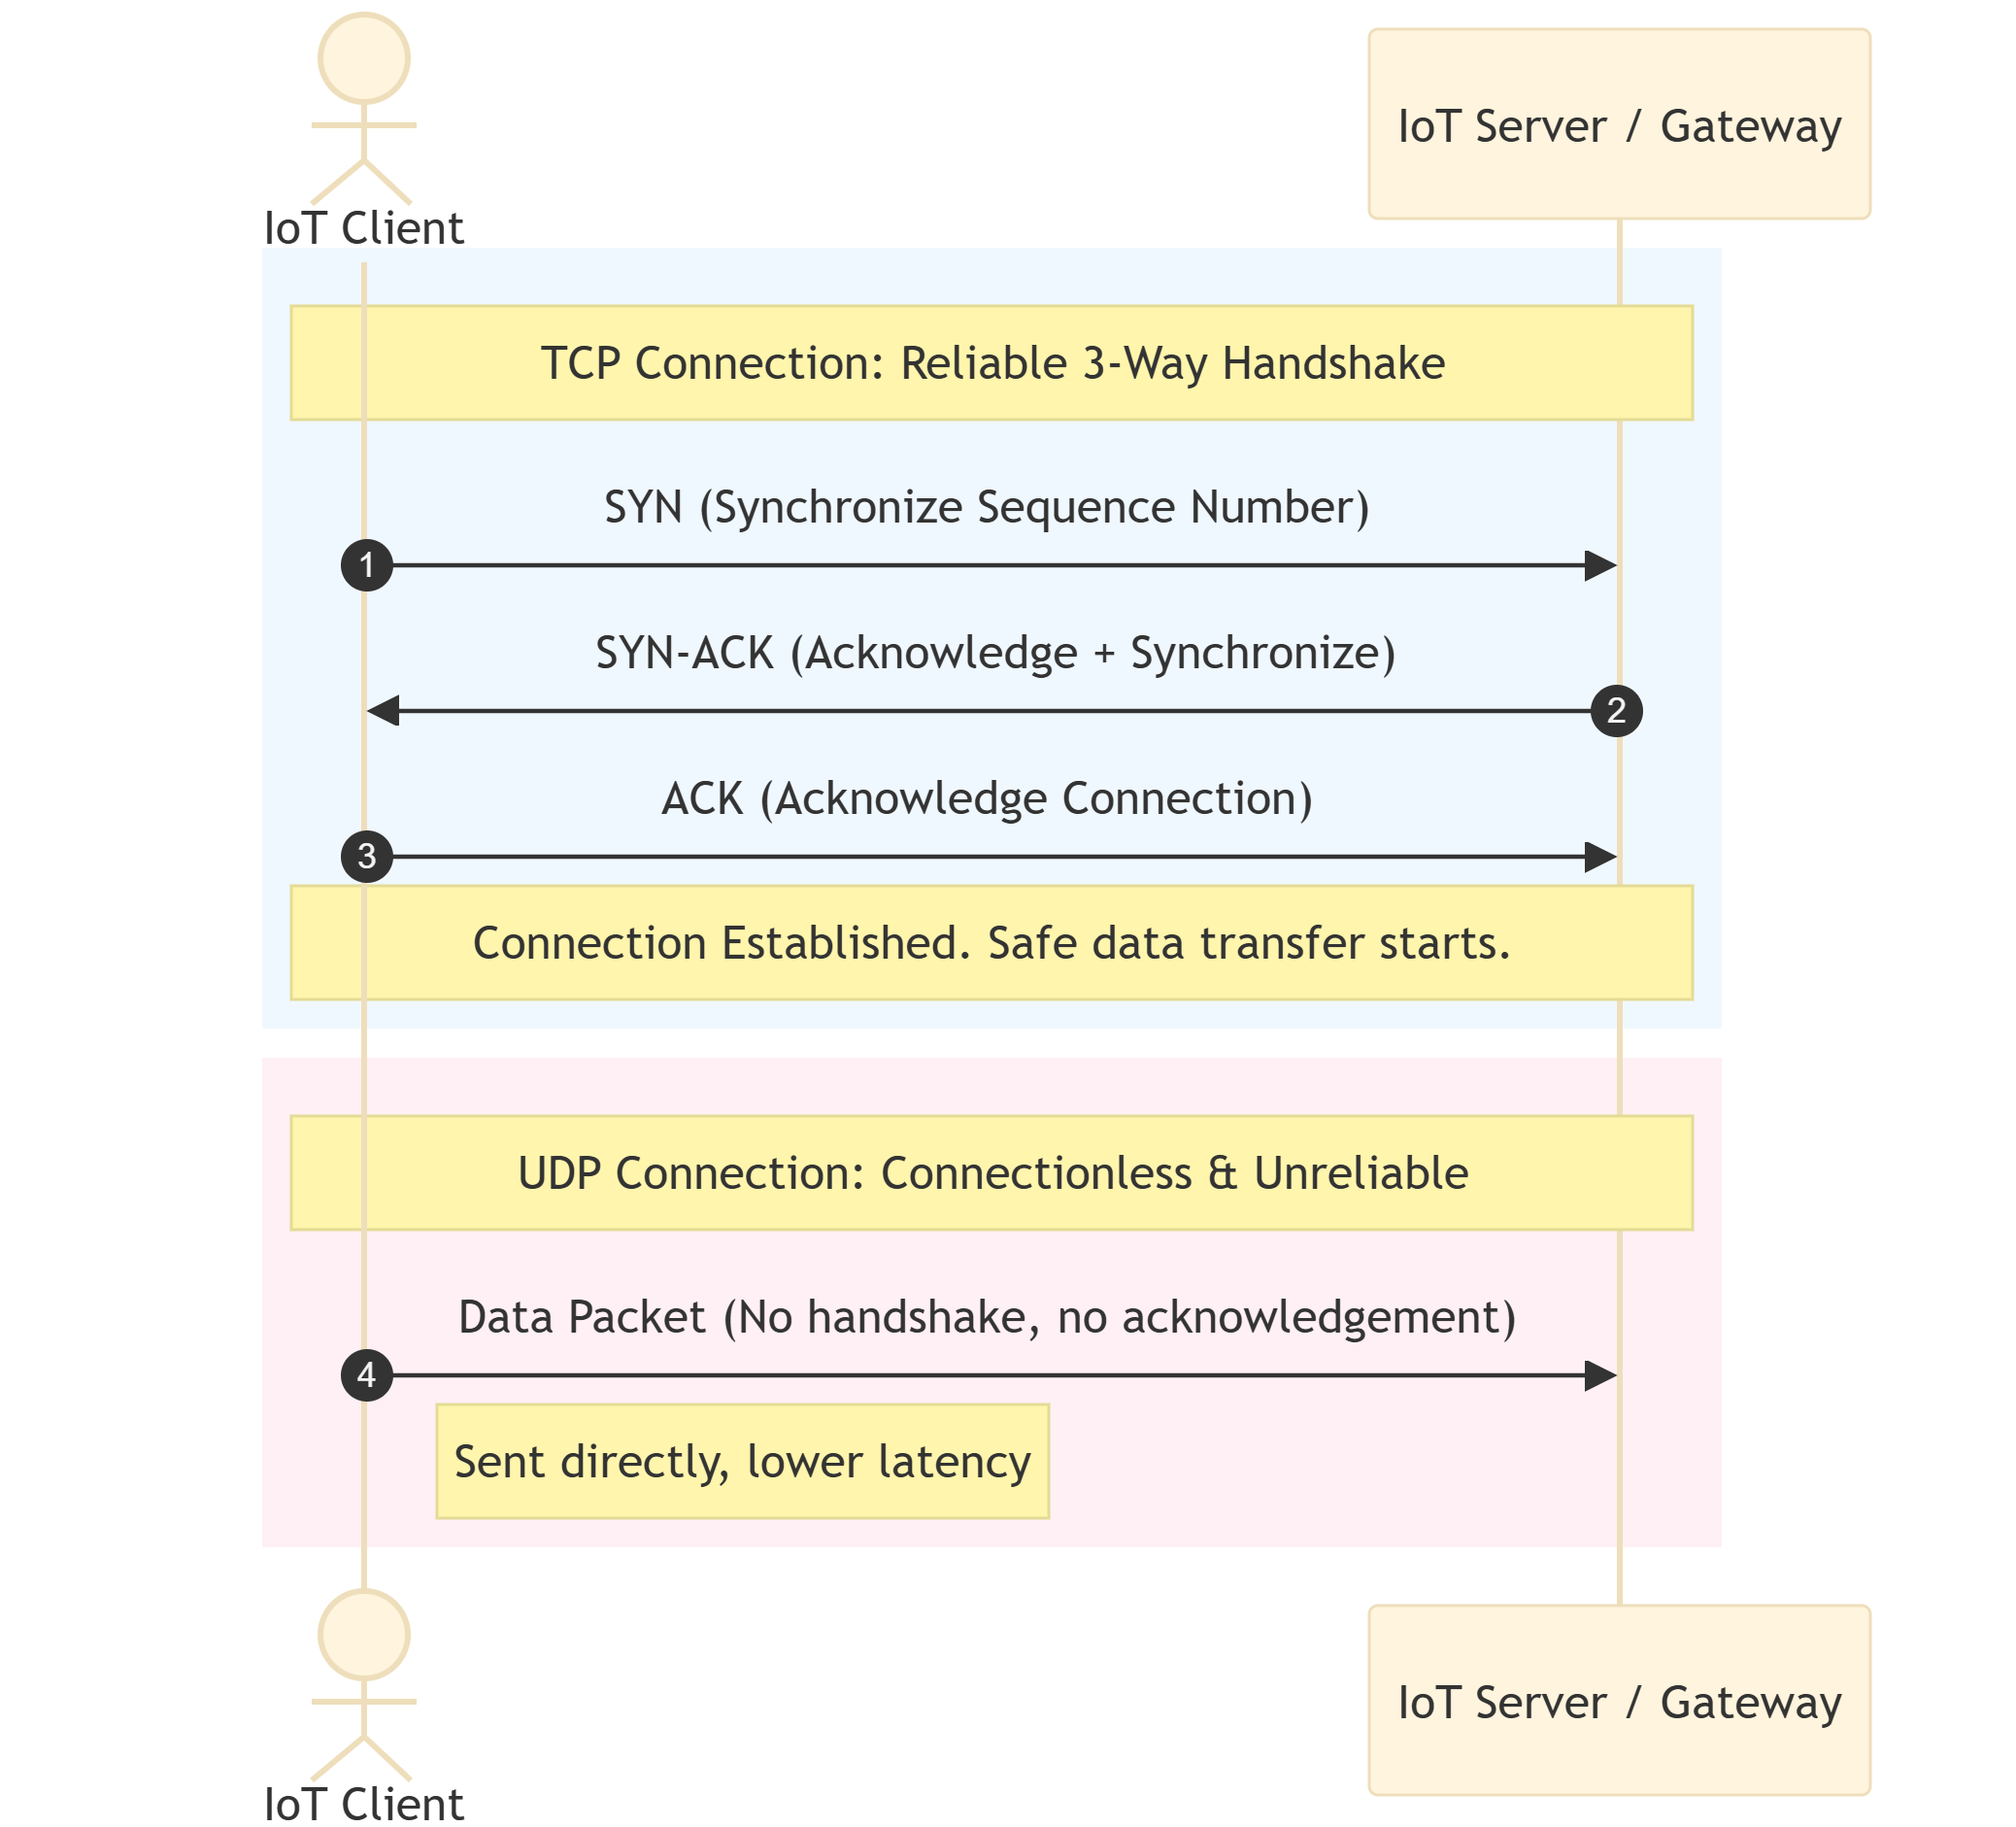
\includegraphics[width=0.75\textwidth,height=0.32\textheight,keepaspectratio]{../Images/chapter_03/tcp_vs_udp.png}
\caption{TCP vs. UDP Protocol Transmission}
\end{figure}


\subsection{1. Comparison: TCP vs. UDP}

\begin{table}[H]
\centering
\begin{tabular}{|p{\dimexpr 0.2\textwidth - 2\tabcolsep - 1.5\arrayrulewidth\relax}|p{\dimexpr 0.4\textwidth - 2\tabcolsep - 1.5\arrayrulewidth\relax}|p{\dimexpr 0.4\textwidth - 2\tabcolsep - 1.5\arrayrulewidth\relax}|}
\hline
Feature / Criteria & TCP (Transmission Control Protocol) & UDP (User Datagram Protocol) \\
\hline
\textbf{Connection Type} & \textbf{Connection-oriented} (requires 3-way handshake). & \textbf{Connectionless} (packets sent independently). \\
\hline
\textbf{Reliability} & Guaranteed delivery (uses ACKs and retransmissions). & Best-effort delivery (no guarantees, packet loss possible). \\
\hline
\textbf{Data Flow Control} & Yes (sliding window controls flow; avoids congestion). & None (sends data as fast as the app generates it). \\
\hline
\textbf{Packet Overhead} & High (20-byte minimum header). & Low (8-byte header). \\
\hline
\textbf{Speed / Latency} & Slower (due to connection setup, sequencing, ACKs). & Fast (no connection overhead, lower latency). \\
\hline
\textbf{Transmission Type} & Byte stream. & Message/Datagram-oriented. \\
\hline
\end{tabular}
\end{table}


\subsection{2. Why UDP is Preferred in Constrained IoT Environments}
Many IoT edge devices are battery-powered, resource-constrained microcontrollers connected over lossy wireless networks. UDP is preferred here because:
\begin{enumerate}
  \item \textbf{Power Conservation:} Establishing a TCP connection requires a 3-way handshake (SYN, SYN-ACK, ACK), and closing it requires a 4-step teardown. This high radio uptime drains batteries. UDP sends data immediately and enters sleep mode.
  \item \textbf{Reduced Overhead:} TCP's 20-byte header is 150\% larger than UDP's 8-byte header. For small sensor payloads (e.g., a 2-byte temperature reading), TCP wastes bandwidth.
  \item \textbf{Low Latency / Real-Time Data:} For streaming parameters (e.g., GPS tracking or live industrial pressure updates), old data is useless. Retransmitting a lost packet (as TCP does) causes lag; UDP simply drops it and waits for the next live reading.
  \item \textbf{Application Layer Control:} Protocols like \textbf{CoAP} implement custom, lightweight reliability directly in the application layer over UDP, avoiding the resource-heavy overhead of transport-layer TCP.
\end{enumerate}


\section{Section 5: IPv6 Protocol in IoT (Q3.4) [5M]}

\subsection{1. Benefits of IPv6 in IoT}
The \textbf{Internet Protocol Version 6 (IPv6)} is replacing IPv4 as the default internet routing layer. Its integration is critical for IoT due to:
\begin{itemize}
  \item   \textbf{Massive Address Space:} IPv6 uses 128-bit addresses, offering $3.4 \times 10^{38}$ unique addresses ($340\text{ undecillion}$). This ensures every single sensor node on earth can have a unique public IP.
  \item   \textbf{SLAAC (Stateless Address Autoconfiguration):} Devices generate their own IP address dynamically using local router advertisements and their MAC address, eliminating the need for a DHCP server.
  \item   \textbf{Header Simplicity \& Router Efficiency:} IPv6 uses a fixed-length header format (40 bytes), allowing routers to process packets faster, reducing latency and gateway power usage.
  \item   \textbf{Built-in IPSec Security:} Cryptographic security (encryption and authentication) is natively supported.
  \item   \textbf{Optimized Multicasting:} Replaces wasteful IPv4 broadcasts with efficient multicast groups, preventing sleeping nodes from waking up for irrelevant broadcast traffic.
\end{itemize}


\subsection{2. Length and Structure of IPv6 Address}
\begin{itemize}
  \item   \textbf{Length:} \textbf{128 bits} (16 bytes).
  \item   \textbf{Representation:} Represented as 8 groups of 4 hexadecimal digits, separated by colons (`:`).
  \item   \textbf{Standard Example:} `2001:0db8:85a3:0000:0000:8a2e:0370:7334`
\end{itemize}

\subsubsection{Structural Breakdown:}
An IPv6 address is split into two halves:
\begin{enumerate}
  \item \textbf{Network Prefix (First 64 bits):} Used for routing packets across the global internet. Typically provided by the ISP and local router.
  \item \textbf{Interface Identifier (Last 64 bits):} Identifies the specific host interface. Frequently derived from the device's physical 48-bit MAC address using the \textbf{EUI-64} format.
\end{enumerate}

\begin{lstlisting}
+---------------------------------------+---------------------------------------+
|        Network Prefix (64 bits)       |      Interface Identifier (64 bits)    |
|  Global Routing + Subnet ID Info      |   Unique Host Address (MAC derived)   |
+---------------------------------------+---------------------------------------+
\end{lstlisting}


\section{Section 6: MAC Address \& Ports (Q3.5) [5M]}

\subsection{1. MAC Address (Physical Address)}
A \textbf{MAC (Media Access Control) address} is a unique, physical hardware identifier assigned to a Network Interface Controller (NIC) during manufacturing.

\begin{itemize}
  \item   \textbf{Length:} \textbf{48 bits} (6 bytes).
  \item   \textbf{Layer:} Operates at the \textbf{Data Link Layer (Layer 2)} of the OSI model.
  \item   \textbf{Format:} Represented as 6 pairs of hexadecimal digits separated by colons or hyphens (e.g., `00:1A:2B:3C:4D:5E`).
\end{itemize}


\subsection{2. MAC Address Structure}
A standard 48-bit MAC address is split into two major parts:

\begin{figure}[H]
\centering
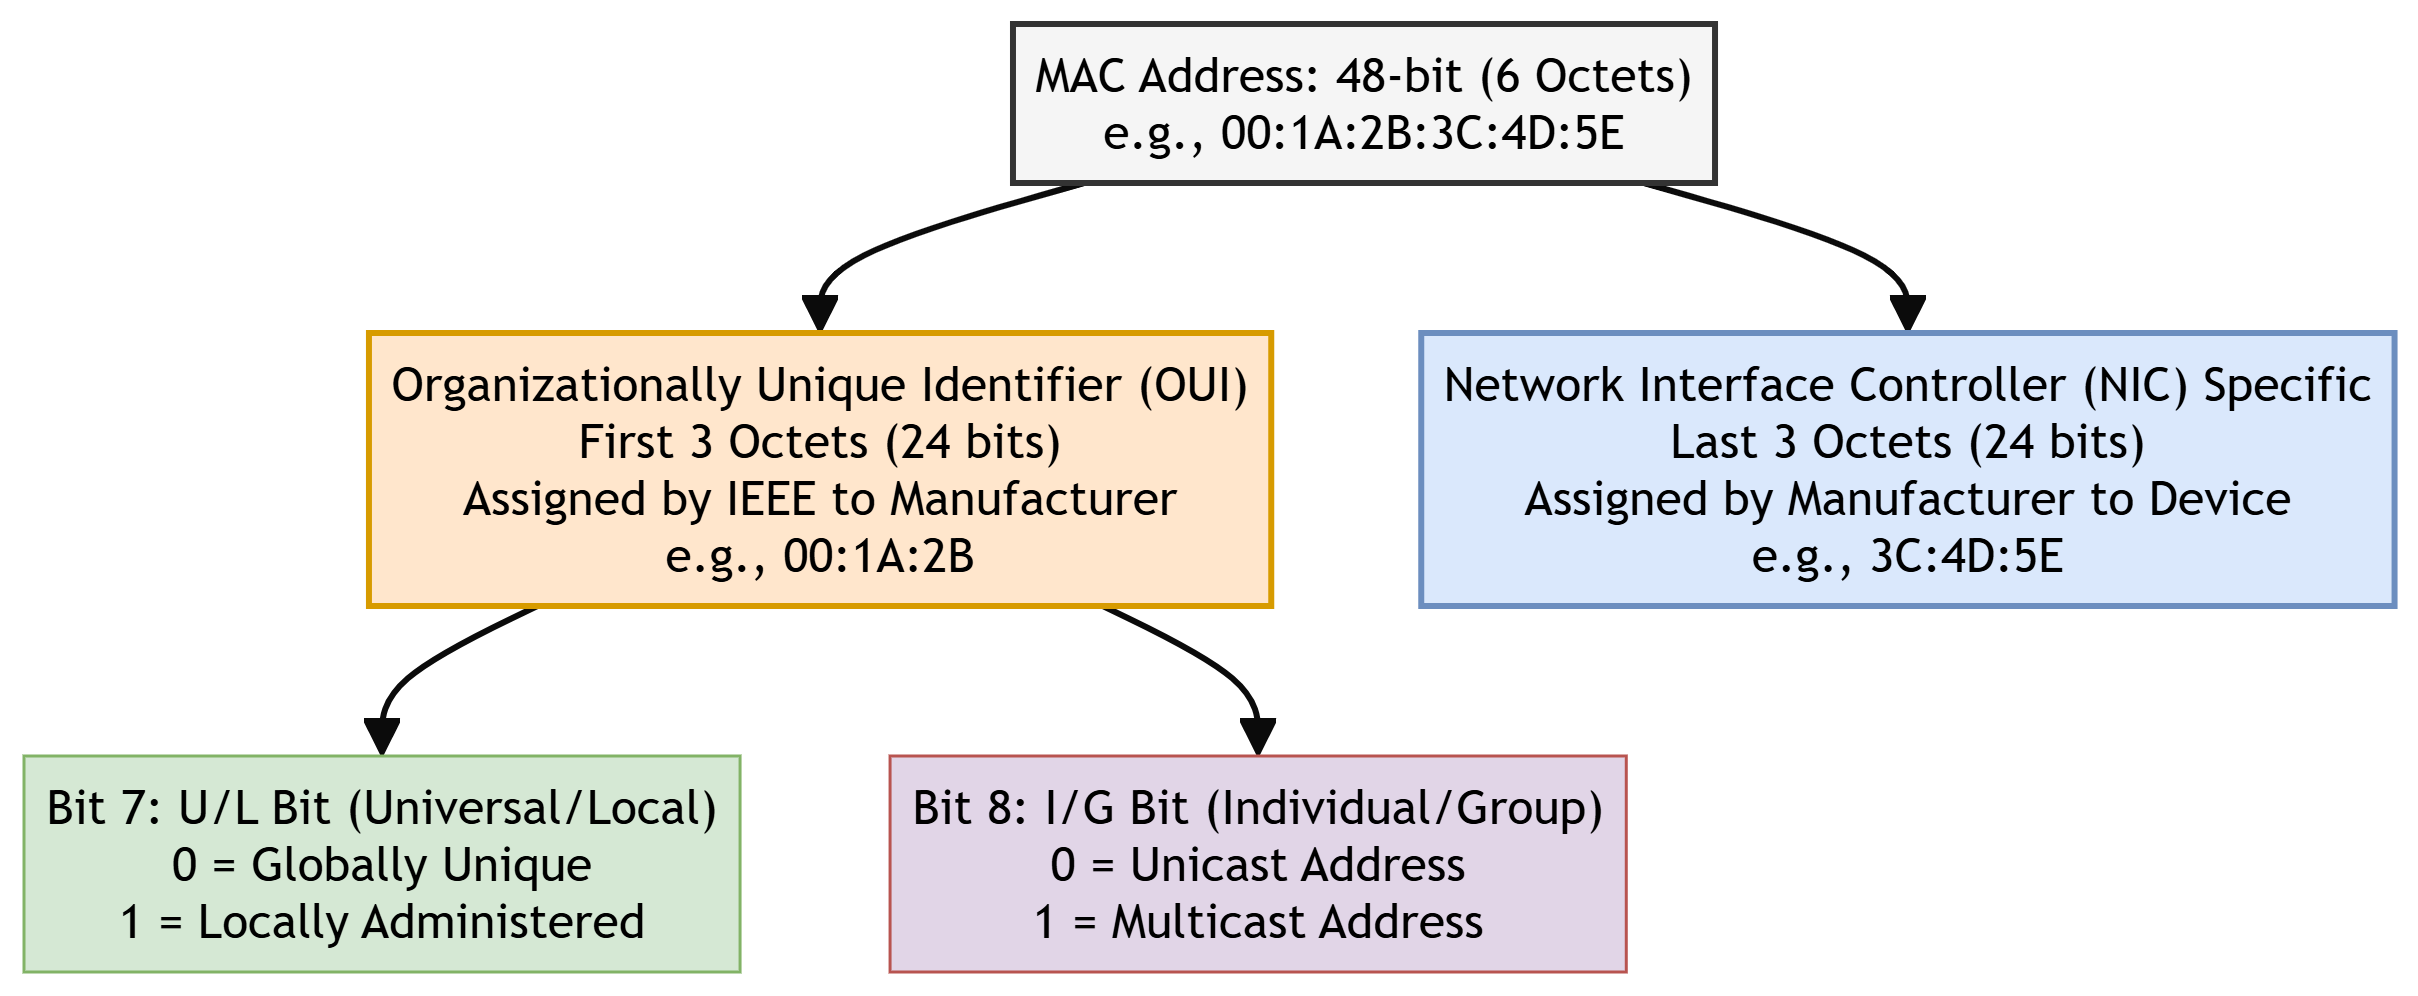
\includegraphics[width=0.75\textwidth,height=0.32\textheight,keepaspectratio]{../Images/chapter_03/mac_address_format.png}
\caption{MAC Address Format Layout}
\end{figure}

\begin{enumerate}
  \item \textbf{Organizationally Unique Identifier (OUI):}
\end{enumerate}
\begin{itemize}
  \item   \textbf{First 24 bits (3 octets):} Assigned by the IEEE Registration Authority to the hardware manufacturer (e.g., Apple, Intel, Espressif).
\end{itemize}
    \textit{   }Bit 7 (U/L Bit):* Specfies whether the address is \textbf{Universally} administered (0) or \textbf{Locally} administered (1).
    \textit{   }Bit 8 (I/G Bit):* Specifies whether the address is \textbf{Individual/Unicast} (0) or \textbf{Group/Multicast} (1).
\begin{enumerate}
  \item \textbf{NIC Specific (Extension Identifier):}
\end{enumerate}
\begin{itemize}
  \item   \textbf{Last 24 bits (3 octets):} Assigned uniquely by the manufacturer to each individual physical chip.
\end{itemize}


\subsection{3. Network Ports}
While IP addresses locate a physical device on a network, \textbf{Ports} are logical endpoints within the operating system that route network traffic to specific software processes or services.

\begin{itemize}
  \item   \textbf{Size:} \textbf{16-bit} unsigned integer (ranging from `0` to `65535`).
  \item   \textbf{Port Classifications:}
\end{itemize}
\begin{enumerate}
  \item \textbf{Well-Known Ports (0 – 1023):} System ports reserved for standard core internet services (e.g., Port `80` for HTTP, Port `443` for HTTPS).
  \item \textbf{Registered Ports (1024 – 49151):} Used by software applications and standard IoT services (e.g., Port `1883` for MQTT unencrypted, Port `8883` for MQTT over TLS).
  \item \textbf{Dynamic / Private Ports (49152 – 65535):} Temporarily assigned to client applications requesting outbound network links.
\end{enumerate}


\section{Section 7: IoT Application Layer Protocols (Q3.6) [15M]}

The Application Layer governs how IoT devices format, structure, and request data. The three key protocols are \textbf{HTTP}, \textbf{CoAP}, and \textbf{MQTT}.

\begin{figure}[H]
\centering
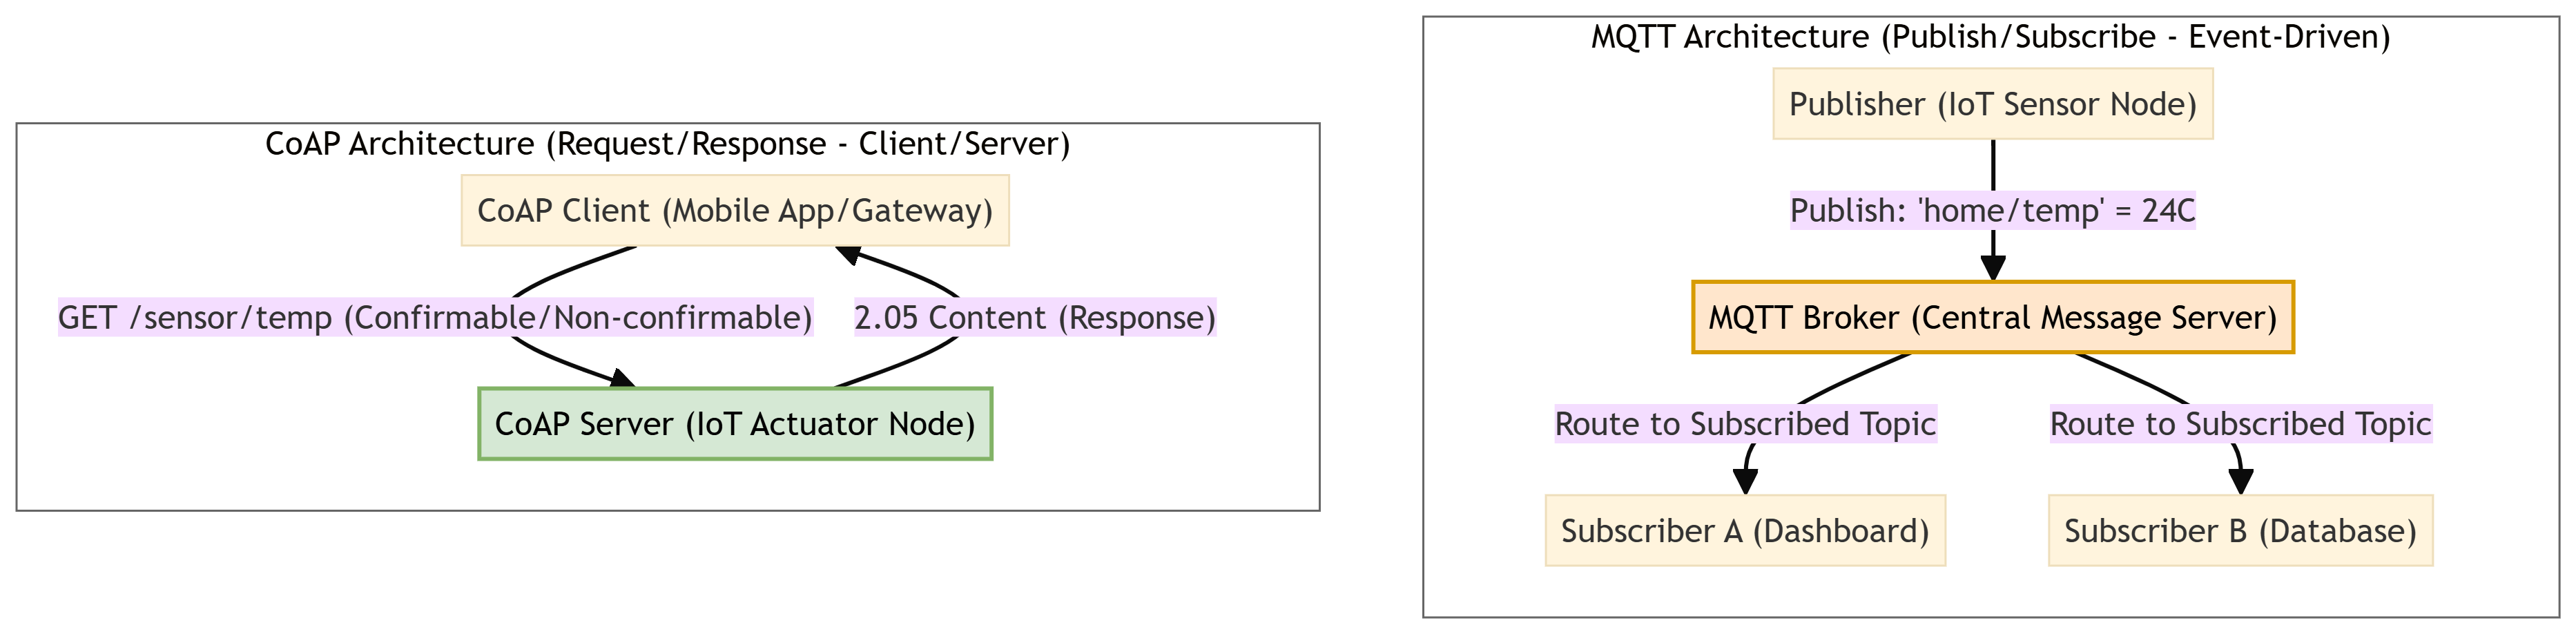
\includegraphics[width=0.75\textwidth,height=0.32\textheight,keepaspectratio]{../Images/chapter_03/mqtt_vs_coap.png}
\caption{MQTT Pub/Sub vs. CoAP Request/Response Architecture}
\end{figure}


\subsection{1. HTTP (Hypertext Transfer Protocol)}
HTTP is the foundation of data communication for the World Wide Web, designed as a synchronous, request-response protocol.

\begin{itemize}
  \item   \textbf{Working Principle:} A client establishes a TCP connection to a server, sends an HTTP request (GET, POST, PUT, DELETE) with verbose ASCII headers, and receives a response back.
  \item   \textbf{Strengths:}
  \item   \textbf{Ubiquity:} Supported by almost all web servers, languages, and firewalls.
  \item   \textbf{Ease of Integration:} Integrates directly with standard corporate databases and cloud storage platforms.
  \item   \textbf{High Security:} Relies on robust HTTPS (TLS) encryption standards.
  \item   \textbf{Limitations in IoT:}
  \item   \textbf{High Overhead:} Headers are in verbose plain text, often exceeding several hundred bytes, which is larger than typical sensor payloads.
  \item   \textbf{Synchronous Pull Model:} The client must poll the server repeatedly to check for updates. Devices cannot receive real-time push events unless they keep a TCP socket open (draining batteries).
  \item   \textbf{Memory Footprint:} Writing a full TCP/HTTP stack requires significant RAM and flash memory.
\end{itemize}


\subsection{2. CoAP (Constrained Application Protocol)}
CoAP is a specialized web transfer protocol designed by the IETF for resource-constrained nodes and networks (RFC 7252).

\begin{itemize}
  \item   \textbf{Working Principle:} CoAP mimics the RESTful design of HTTP (GET/POST/PUT/DELETE) but runs over lightweight \textbf{UDP} instead of TCP. It uses highly compressed, fixed-length \textbf{binary headers} (minimum 4 bytes).
  \item   \textbf{Strengths:}
  \item   \textbf{Extremely Low Overhead:} Minimizes header size, reducing packet fragmentation over low-power networks.
  \item   \textbf{Designed for Microcontrollers:} Can easily run on chips with under 10 KB of RAM.
  \item   \textbf{Supports Observation Mode:} A CoAP client can "observe" a resource. The server will push updates to the client whenever the state changes, eliminating the need for periodic client polling.
  \item   \textbf{Limitations:}
  \item   \textbf{Transport Unreliability:} Because UDP is connectionless, CoAP must handle lost packets manually using built-in Confirmable (CON) and Non-confirmable (NON) message flags.
  \item   \textbf{NAT Traversal Issues:} Firewalls and NAT gateways frequently block inbound UDP traffic, making it hard to contact sleep-wake nodes directly from the public internet.
\end{itemize}


\subsection{3. MQTT (Message Queuing Telemetry Transport)}
MQTT is an extremely lightweight, broker-based publish/subscribe messaging protocol designed by IBM in 1999 (now an OASIS standard).

\begin{itemize}
  \item   \textbf{Working Principle:} Devices do not communicate directly. Instead, they connect to a central \textbf{MQTT Broker} via TCP. Clients publish data to specific text-based \textbf{Topics} (e.g., `home/kitchen/temp`), and other clients subscribe to those topics to receive real-time updates.
  \item   \textbf{Strengths:}
  \item   \textbf{Event-Driven (Pub/Sub):} Separates the data publisher from the subscriber, ideal for one-to-many communications.
  \item   \textbf{Low Bandwidth:} The binary header is tiny (minimum \textbf{2 bytes}).
  \item   \textbf{Three Quality of Service (QoS) Levels:}
\end{itemize}
\begin{enumerate}
  \item \textit{QoS 0 (At most once):} Minimal overhead; packet sent without confirmation (fire and forget).
  \item \textit{QoS 1 (At least once):} Guarantees delivery by requiring an acknowledgement, but duplicates are possible.
  \item \textit{QoS 2 (Exactly once):} Highest reliability; uses a 4-step handshake to guarantee data arrives exactly once.
\end{enumerate}
\begin{itemize}
  \item   \textbf{LWT (Last Will \& Testament):} The broker automatically notifies other subscribers if a client disconnects unexpectedly.
  \item   \textbf{Limitations:}
  \item   \textbf{Central Broker Dependency:} If the central broker fails, the entire IoT network goes offline (single point of failure).
  \item   \textbf{TCP Keep-Alives:} Requires clients to send periodic "ping" packets to keep the TCP connection alive, which can drain battery reserves over time.
  \item   \textbf{No Native Data Security:} Relies on transport layer security (TLS/SSL), which increases encryption overhead on small microcontrollers.
\end{itemize}


\subsection{4. Comparison: HTTP vs. CoAP vs. MQTT}

\begin{table}[H]
\centering
\begin{tabular}{|p{\dimexpr 0.18\textwidth - 2\tabcolsep - 1.5\arrayrulewidth\relax}|p{\dimexpr 0.27\textwidth - 2\tabcolsep - 1.5\arrayrulewidth\relax}|p{\dimexpr 0.27\textwidth - 2\tabcolsep - 1.5\arrayrulewidth\relax}|p{\dimexpr 0.28\textwidth - 2\tabcolsep - 1.5\arrayrulewidth\relax}|}
\hline
Feature / Criteria & HTTP & CoAP & MQTT \\
\hline
\textbf{Architecture Model} & Client-Server (Request-Response) & Client-Server (Request-Response) & Broker-Client (Publish-Subscribe) \\
\hline
\textbf{Transport Layer} & TCP & UDP & TCP \\
\hline
\textbf{Header Format} & Verbose ASCII Text (100s of bytes) & Compressed Binary (min 4 bytes) & Compact Binary (min 2 bytes) \\
\hline
\textbf{Communication Mode} & Synchronous (Pull) & Asynchronous (Push/Pull via Observe) & Asynchronous (Event-Driven Push) \\
\hline
\textbf{Resource Constraints} & High (Not suitable for node chips) & Low (Excellent for microcontrollers) & Low to Medium (Broker handles load) \\
\hline
\textbf{QoS Support} & None (Relies on TCP layer) & Basic (CON/NON messages) & Rich (QoS 0, QoS 1, QoS 2) \\
\hline
\textbf{Real-time Push} & Hard (requires polling/websockets) & Easy (via Observation mode) & Native (via Publish/Subscribe) \\
\hline
\end{tabular}
\end{table}


\subsection{5. Conclusion}
\begin{itemize}
  \item   Use \textbf{HTTP} for cloud-to-cloud communications and web dashboard interfaces where bandwidth and power are unlimited.
  \item   Use \textbf{CoAP} for point-to-point operations on highly constrained nodes (e.g., smart utility meters) communicating over lossy networks.
  \item   Use \textbf{MQTT} for large-scale networks with many-to-many communication needs, real-time push requirements, and fluctuating network reliability (e.g., smart home automations).
\end{itemize}


\section{Section 8: Weightless Protocol (Q3.7) [5M][]}

\subsection{1. Definition \& Overview}
The \textbf{Weightless} protocol is an open standard LPWAN (Low-Power Wide-Area Network) communication protocol specifically optimized for machine-to-machine (M2M) and IoT communications. It operates in the \textbf{sub-GHz TV White Space (TVWS)} spectrum (the unused frequencies between active television channels), offering long-range and low-power operations.

\subsection{2. Core Features of Weightless}
\begin{itemize}
  \item   \textbf{TV White Spaces Utilization:} Operates in UHF/VHF bands (typically 470–790 MHz), which provide superior signal penetration through walls and obstacles compared to 2.4 GHz bands.
  \item   \textbf{Narrowband Technology:} Employs narrow carrier bands (e.g., 180 kHz) to achieve high receiver sensitivity and long ranges (up to 10 km in urban areas, 30 km in line-of-sight).
  \item   \textbf{Symmetric Links:} Offers balanced downlink and uplink data rates, which is crucial for over-the-air firmware updates and command delivery.
  \item   \textbf{High Spectral Efficiency:} Uses techniques like TDMA (Time Division Multiple Access) and FDMA (Frequency Division Multiple Access) to handle thousands of endpoints per base station.
  \item   \textbf{Low Power Consumption:} Uses highly optimized sleep states, enabling nodes to run for over 10 years on a single AA battery.
\end{itemize}


\section{Section 9: Edge, Fog, Mist, and Cloud Computing (Q3.8) [5M][]}

To address latency, bandwidth constraints, and privacy issues, modern IoT architectures distribute computing tasks across multiple layers between the physical device and the remote cloud:

\begin{lstlisting}
[ Physical World ] 
       │
       ▼
 [ Mist Layer ]   ──► Computing on microcontrollers/sensors (closest to data)
       │
       ▼
 [ Edge Layer ]   ──► Computing on local gateways/controllers (same LAN)
       │
       ▼
 [ Fog Layer ]    ──► Computing on regional nodes/routers (local area network)
       │
       ▼
 [ Cloud Layer ]  ──► Computing on remote data centers (highest capacity)
\end{lstlisting}

\subsection{1. Detailed Layer Comparison}

\begin{table}[H]
\centering
\begin{tabular}{|p{\dimexpr 0.16\textwidth - 2\tabcolsep - 1.5\arrayrulewidth\relax}|p{\dimexpr 0.21\textwidth - 2\tabcolsep - 1.5\arrayrulewidth\relax}|p{\dimexpr 0.21\textwidth - 2\tabcolsep - 1.5\arrayrulewidth\relax}|p{\dimexpr 0.21\textwidth - 2\tabcolsep - 1.5\arrayrulewidth\relax}|p{\dimexpr 0.21\textwidth - 2\tabcolsep - 1.5\arrayrulewidth\relax}|}
\hline
Criteria / Feature & Mist Computing & Edge Computing & Fog Computing & Cloud Computing \\
\hline
\textbf{Proximity to User/Device} & On-device (physical node). & Immediate proximity (gateway level, local LAN). & Near proximity (LAN/MAN node, network edge). & Remote (internet cloud servers). \\
\hline
\textbf{Processing Power} & Very low (microcontrollers). & Medium (gateways, industrial controllers). & High (regional servers/routers). & Virtually unlimited (data centers). \\
\hline
\textbf{Latency} & Extremely low ($<$ 1 ms). & Very low (1–10 ms). & Low (10–100 ms). & High (100–500 ms+). \\
\hline
\textbf{Bandwidth Usage} & None (data processed where sensed). & Low (aggregates and filters before sending). & Medium (regional data aggregation). & High (requires streaming all raw data). \\
\hline
\textbf{Primary Use Case} & Basic raw filtering, sensor self-calibrations. & Real-time local safety shutdown, video processing. & Local area traffic coordination, smart grid substations. & Long-term trend forecasting, training ML models. \\
\hline
\end{tabular}
\end{table}

